\begin{figure}%
    \centering
    \subfloat[]{{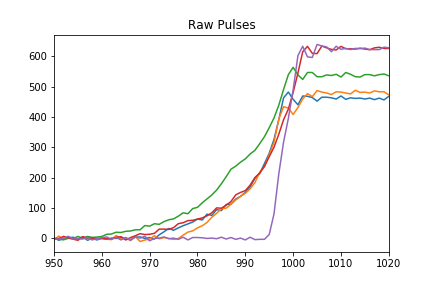
\includegraphics[width=7cm]{./figures/tenevents_rawdata.pdf} }}%
    \quad
    \subfloat[]{{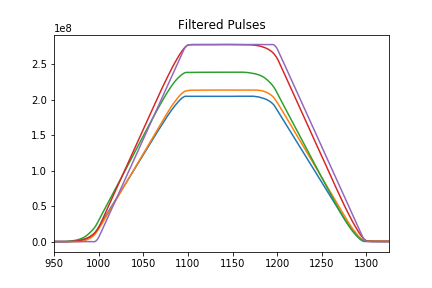
\includegraphics[width=7cm]{./figures/tenevents_filtered.pdf} }}%
    \caption{In figure (a) 5 sample events are shown. In figure (b) are the five signals after the application of a trapezoidal filter with a gap time and peaking time of 1 $\mu$s. Signals of the same color correspond to one another. Note that the time interval on both plots in in ADC samples, which are each 10 ns apart in time.}%
    \label{fig:signals}%
\end{figure}

Five signals were chosen from the ${}^{137}{Cs}$ data set. The raw signals are plotted in \ref{fig:signals}, after a baseline correction. The resultant signals after usage of the trapezoidal filter with a gap time and peaking time of 1 $\mu$s are also plotted. The correlation between amplitudes can be seen. The signal in purple exhibits ideal behavior, with sharp edges and a flat top. This signal corresponds to the unfiltered signal with the fastest rise-time. All of the charge is collected quickly and the unfiltered signal more closely resembles an ideal step function. The red signal is of the same amplitude but has a longer rise time. As expected, the resultant trapezoid is less ideal, showing more curved corners and more variation in amplitude in the flat top region. These effects can lead to degraded energy resolution.

If the gap time of a filter is too small, ballistic deficit can be seen. This happens when filter rise time and gap time are not large enough to allow full charge collection. Making the gap time longer negates this effect. However, making the gap time too long can give the filter worse noise performance. 

In this implementation the effects of ballistic deficit on energy resolution can be seen. For small gap times, the peak position is shifted down in energy. Also, the peak is broader and tends to have low-energy tailing. Some of this is likely due to ballistic deficit. For gap times greater than a certain amount ($\approx$)250 ns, no significant variation in energy resolution with increasing gap time was observed. This value corresponds well to the expected value for the maximum transit time for charge carriers expected in a small ($\approx$ 4.5 cm diameter) coaxial HPGe detector \cite{Knoll} ),

A plot of resolution as a function of gap time is shown in \ref{gap}.

A plot of resolution as a function of peaking time is shown in \ref{peak}. The optimal peaking time is $\approx $ 10 $\mu$s. This is a reasonable optimal peaking time for such a system. From \ref{peak} we can see that our system has relatively low parallel noise (typically dominated by detector leakage current) and high series noise (dominated by capacitance) in the examined range of peaking times.

\begin{figure}[]
\begin{centering}
\includegraphics[width=0.8\textwidth]{gap_optimization_co.pdf}
\caption{Energy resolution as a function of gap time for the 1173 keV peak in ${}^{60}$Co. The peaking time was kept fixed at 500 ns. The minimum fwhm occurs at a gap time of 450 ns. The errors shown only account for fitting errors.}
\label{gap}
\end{centering}
\end{figure}
\vspace{5mm}

\begin{figure}[]
\begin{centering}
\includegraphics[width=0.8\textwidth]{peak_optimization_co.pdf}
\caption{Energy resolution as a function of peaking time for the 1173 keV peak in ${}^{60}$Co. The gap time was kept fixed at 450 ns. The minimum fwhm occurs are a peaking time of 10 $\mu$s. The errors shown only account for fitting errors.}
\label{peak}
\end{centering}
\end{figure}
\vspace{5mm}

\begin{figure}[]
\begin{centering}
\includegraphics[width=0.8\textwidth]{fwhm_vs_energy.pdf}
\caption{Energy resolution as a function of gamma energy is plotted. Error bars account for fitting errors. These error bars are smaller than the markers and thus not visible.}
\label{peak}
\end{centering}
\end{figure}
\vspace{5mm}

The Fano factor, the ratio of the observed variance in the number of charge carriers to the predicted variance in number for a Poisson process, can now be calculated.

\begin{equation}
(FWHM)^{2}_{overall} = (FWHM)^{2}_{statistical}+ (FWHM)^{2}_{electronic} + (FWHM)^{2}_{chargeloss}
\end{equation}

Assuming that charge loss is negligible in our system,

\begin{equation}
(FWHM)^{2}_{statistical} = (FWHM)^{2}_{overall} - (FWHM)^{2}_{electronic}
\end{equation}
\begin{equation}
(FWHM)^{2}_{statistical} = 2.35 \times \sqrt{F \epsilon E}
\end{equation}
where $F$ is the Fano factor, $E$ is the energy of the gamma-ray, and $\epsilon$ is the energy needed to create an electron hole pair. Thus,
\begin{equation}
F = ((FWHM)^{2}_{overall} - (FWHM)^{2}_{electronic}) \frac{1}{2.35 \epsilon E}
\end{equation}

Using this calculation, a fano factor was calculated for each of four calibration peaks (${}^{241}Am$ 59.536 keV, ${}^{137}Cs$ 661.615keV, ${}^{60}Co$ 1173.231keV , ${}^{60}Co$ 1332.508 keV)
  
A pulser input was used in each data set, with varying energy. The pulser peak is meant to provide a measure of electronic noise since the resolution of the pulser peak is decoupled from charge loss, carrier statistics, and other detector-dependent noise sources. There was some variation in the pulser peak resolution with energy, likely due to background and imperfect fitting. The average pulser resolution was used in calculating the Fano factor. Of the four calculated values, the one corresponding to the ${}^{241}Am$ peak was very different than the other values. This is likely because the background for this peak is the most considerable and leads to errors in peak fitting with a simple linear background. This value was discarded. An average of the other three fano factor values gives:

\begin{equation}
F = 0.094 \pm 0.026
\end{equation}

Experimentally the Fano factor has been found to be $\approx 0.129$  \cite{Knoll}. CITATION